\section{Konzept} \label{eth_konzept}

Der Ablauf des Spiels ist mit dem Ablauf aus dem Bitcoin Kapitels nahezu identisch. Die Unterschiede sind, dass das gesamte Spiel vom Nutzer initiiert wird und die Glücksspielanwendung ausschließlich den Spielstatus anzeigt. Dies führt dazu, dass die Spieler keinerlei Vertrauen in die Glücksspielanwendung setzen müssen. Statt aufgrund leichter Überprüfbarkeit die letzte numerische Stelle des Blockhashs für die Gewinnerauswahl zu nutzen, kann bei Ethereum der gesamten Blockhash zur Gewinnerauswahl genutzt werden. Der Spieler kann aufgrund der Konsensregeln darauf vertrauen, dass das Ethereum Netzwerk die Ausführung des Contract Codes korrekt durchführt und die modulo Funktion zur Gewinnerauswahl korrekt berechnet. Die Nutzung des gesamten Blockhashs als Zufallsquelle ermöglicht Töpfe beliebiger Größe. 
Der Ablauf des Spiels lässt sich durch den folgenden Zustandsautomat beschreiben.

\begin{figure}[H]
\centering
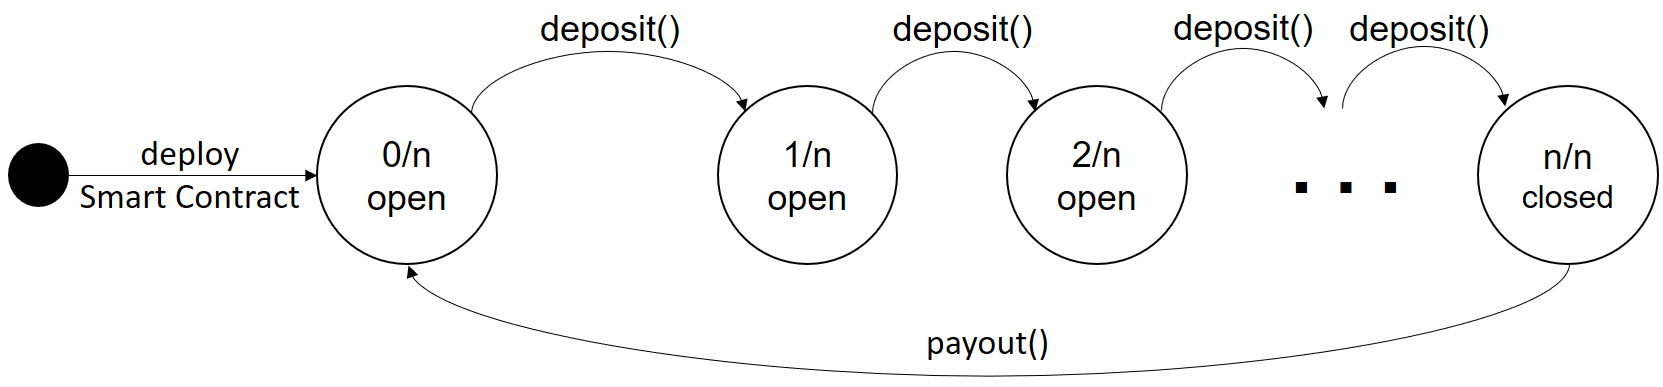
\includegraphics[width=1\linewidth]{Figures/umsetzung_eth/smart_contract_automat_idea}
\decoRule
\caption{Smart Contract Automat}
\label{fig:smart_contract_automat_idea}
\end{figure}

Durch den Aufruf der \code{deploy} Funktion wir der Smart Contract in einer Transaktion an das Netzwerk gesendet und in die Blockchain aufgenommen. Innerhalb des Smart Contracts sind der Einzahlungsbetrag und die Anzahl Teilnehmer \code{n} fest definiert. Ab diesem Moment kann der Code des Smart Contract nicht mehr verändert werden. Im initialen Zustand ist der Topf leer, da noch kein Spieler eingezahlt hat. Nun können genau \code{n} Einzahlungen von Spielern durch den Aufruf der \code{deposit} Funktion getätigt werden. Dazu benötigen die Spieler lediglich einen Ethereum Client, ausreichend Ether\footnote{Einzahlungsbetrags plus Transaktionskosten und optimaler Weise genug Ether für das Bezahlen der \code{payout} Funktion.} und die Adresse des Smart Contracts. Ab dem Zeitpunkt an dem der Smart Contract die letzte Einzahlungstransaktion empfängt, wird der Topf geschlossen und die Blocknummer für die Gewinnerauswahl festgelegt. Der Block der den Gewinner des Topfs entscheidet, muss in der Zukunft liegen und darf nicht vorher bekannt sein, da sonst Betrugsmöglichkeiten entstehen. Zum Zeitpunkt der letzten Einzahlungstransaktion ist es nicht möglich aus dem Smart Contract Code heraus auf den Blockhash des Blocks zuzugreifen in dem sich die letzte Einzahlungstransaktion befindet. Dies liegt daran, dass die Miner das Resultat der Zustandsveränderung aller Transaktionen des Blockes in den Blockheader schreiben müssen und erst anschließend den Blockhash berechnen. Die Transaktionen, die den Contract Code ausführen, können somit nicht auf den Blockhash zugreifen, da dieser zum Zeitpunkt der Codeausführung noch nicht feststeht. Es ist somit unumgänglich nach der letzten Einzahlungstransaktion eine Funktion aufzurufen, die den Gewinner auswählt, die Auszahlung startet und den Topf anschließend für ein neues Spiel wieder öffnet. Dies ist die in Abbildung \ref{fig:smart_contract_automat_idea} gezeigte \code{payout} Funktion.